\documentclass{beamer}

\usepackage[utf8]{inputenc} % Set Encoding
\usepackage[T1]{fontenc} % Enable cyrillic fonts
\usepackage{fontspec} % Using custom fonts (requires -xelatex flag)
\usepackage{graphicx} % For image insertions
\usepackage{float} % For positioning
\usepackage[section]{placeins}
\usepackage{fontspec}
\usepackage{minted} % For code listing

\setmainfont[
  Ligatures=TeX,
  Extension=.otf,
  BoldFont=cmunbx,
  ItalicFont=cmunti,
  BoldItalicFont=cmunbi,
]{cmunrm}
\setsansfont[
  Ligatures=TeX,
  Extension=.otf,
  BoldFont=cmunsx,
  ItalicFont=cmunsi,
]{cmunss}

\setbeamertemplate{footline}[frame number]
\beamertemplatenavigationsymbolsempty
\setlength{\parskip}{1em}

\graphicspath{{./pics}}

\title{An Image is Worth 16x16 Words}
\subtitle{Міждисциплінарний курсовий проект}
\author[Соколенко]{
    Соколенко Дмитро Олександрович
}
\institute[ХНУРЕ]{ІТШІ-18-1 
    \\ \vspace{0.4cm}
    Керівник: Вітько О. В.
}
\date{Харків 2021}

\begin{document}
\frame{\titlepage}

\begin{frame}
    \frametitle{Вступ}
    Архітектура трансформера вже стала стандартом для
    вирішення задач природної обробки мови.

    Проте її застосування до обробки зображень залишаються
    обмеженими.
    
\end{frame}

\begin{frame}
    \frametitle{Основи трансформера}
    \begin{itemize}
        \item Не використовує рекурентність
        \item Не використовує згортковість
        \item Повністю полягаться на механізм уваги
        \item Легко паралелізується
    \end{itemize}

\end{frame}

\begin{frame}
    \frametitle{Механізм уваги}
    \begin{figure}[H]
        \centering
        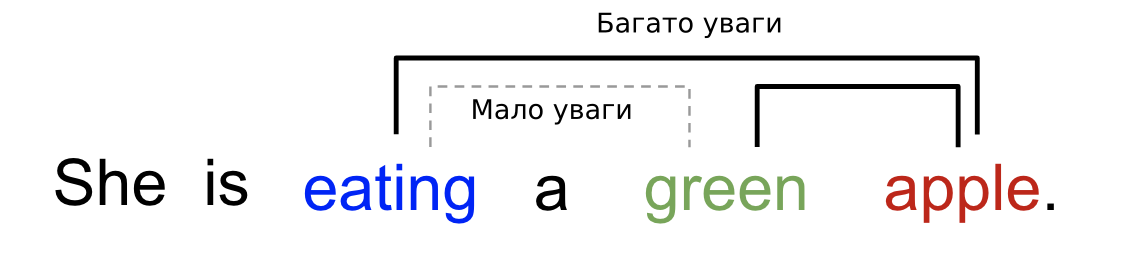
\includegraphics[width=0.75\textwidth]{sentence-example-attention.png}
    \end{figure}
    Увага оцінює, наскільки сильно один елемент
    співвідноситься з іншими елементами, і приймає значення
    зваженої суми

    \begin{equation*}
        c_t = \sum^n_{i=1}\alpha_{t,i} h_i
    \end{equation*}
    
\end{frame}

\begin{frame}
    \frametitle{Багатоголова увага}

    У трансформері увага виражається формулою:
    \begin{equation*}
        \text{Attention(Q,K,V)} = \text{softmax}(\frac{QK^T}{\sqrt{n}})V
    \end{equation*}
    Де
    \begin{equation*}
        Q=XW_Q, K=XW_K, V=XW_V
    \end{equation*}

    Багатоголова увага є конкатенацією виходів декількох головок:
    \begin{gather*}
    \begin{aligned}
        \text{MultiHead}(Q,K,V)= [\text{head}_1; ...; \text{head}_h]W^O \\
        \text{head}_i = \text{Attention}(QW^Q_i, KW^K_i, VW^V_i)
    \end{aligned}
        \end{gather*}
\end{frame}

\begin{frame}
    \frametitle{Багатоголова увага}
    \begin{figure}[H]
        \centering
        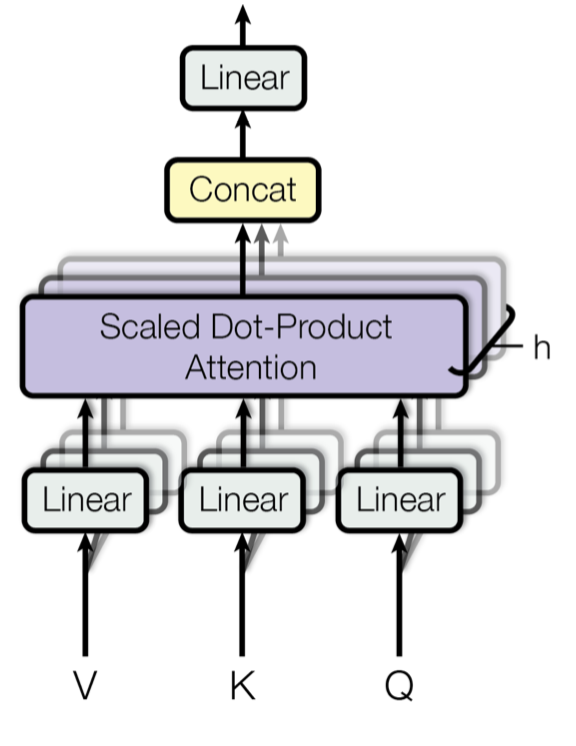
\includegraphics[width=0.5\textwidth]{multi-head-attention.png}
    \end{figure}

\end{frame}

\begin{frame}
    \frametitle{Архітектура трансформера для машинного перекладу}
    \begin{figure}[H]
        \centering
        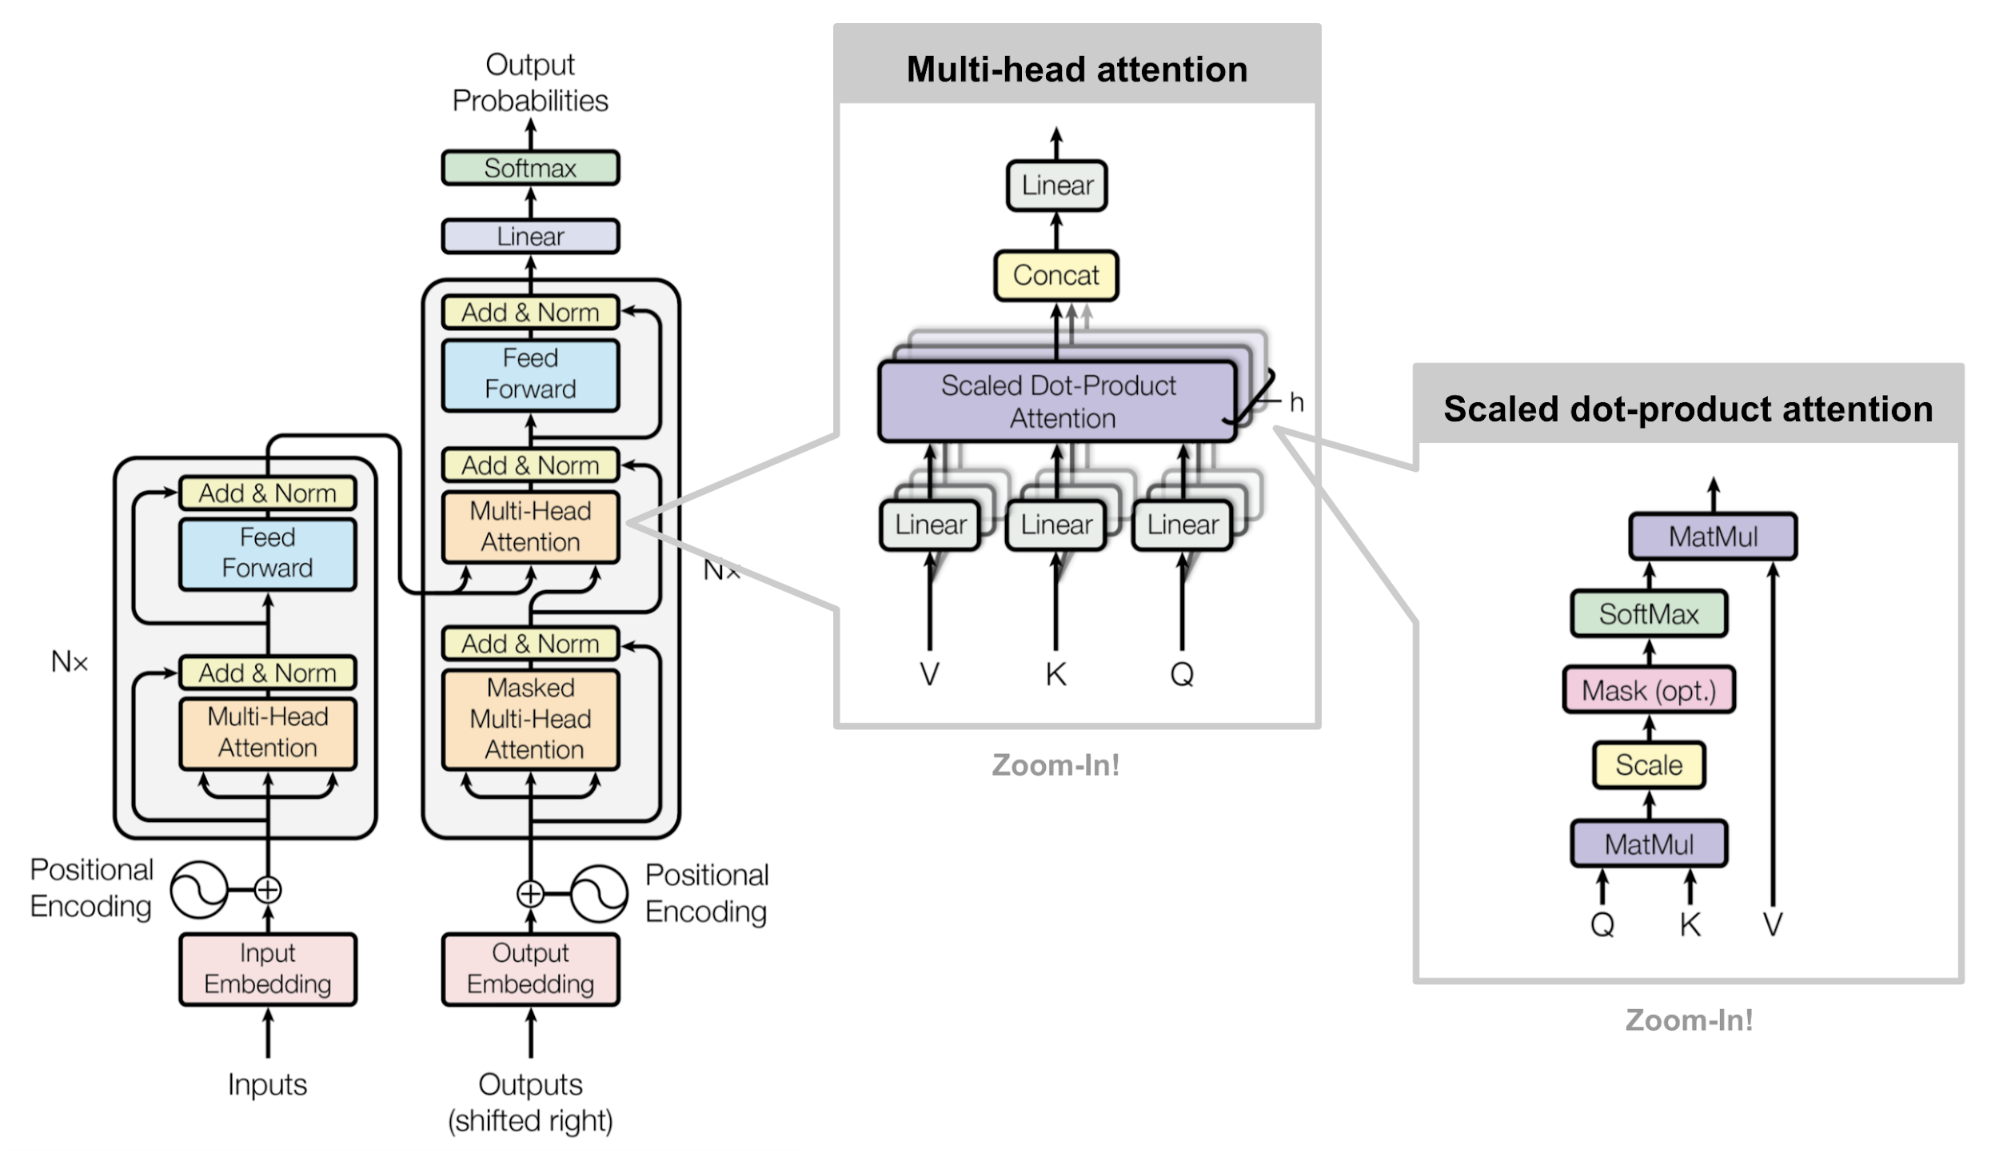
\includegraphics[width=1\textwidth]{transformer.png}
    \end{figure}
    
\end{frame}

\begin{frame}
    \frametitle{Vision Transformer}
    \begin{itemize}
        \item Максимально точно дотримується архітектури
        оригінального трансформера
        \item Використовується для класифікації зображень
        \item Представляє зображення як послідовність різних регіонів
    \end{itemize}
    
\end{frame}

\begin{frame}
    \frametitle{Vision Transformer}
    \begin{figure}[H]
        \centering
        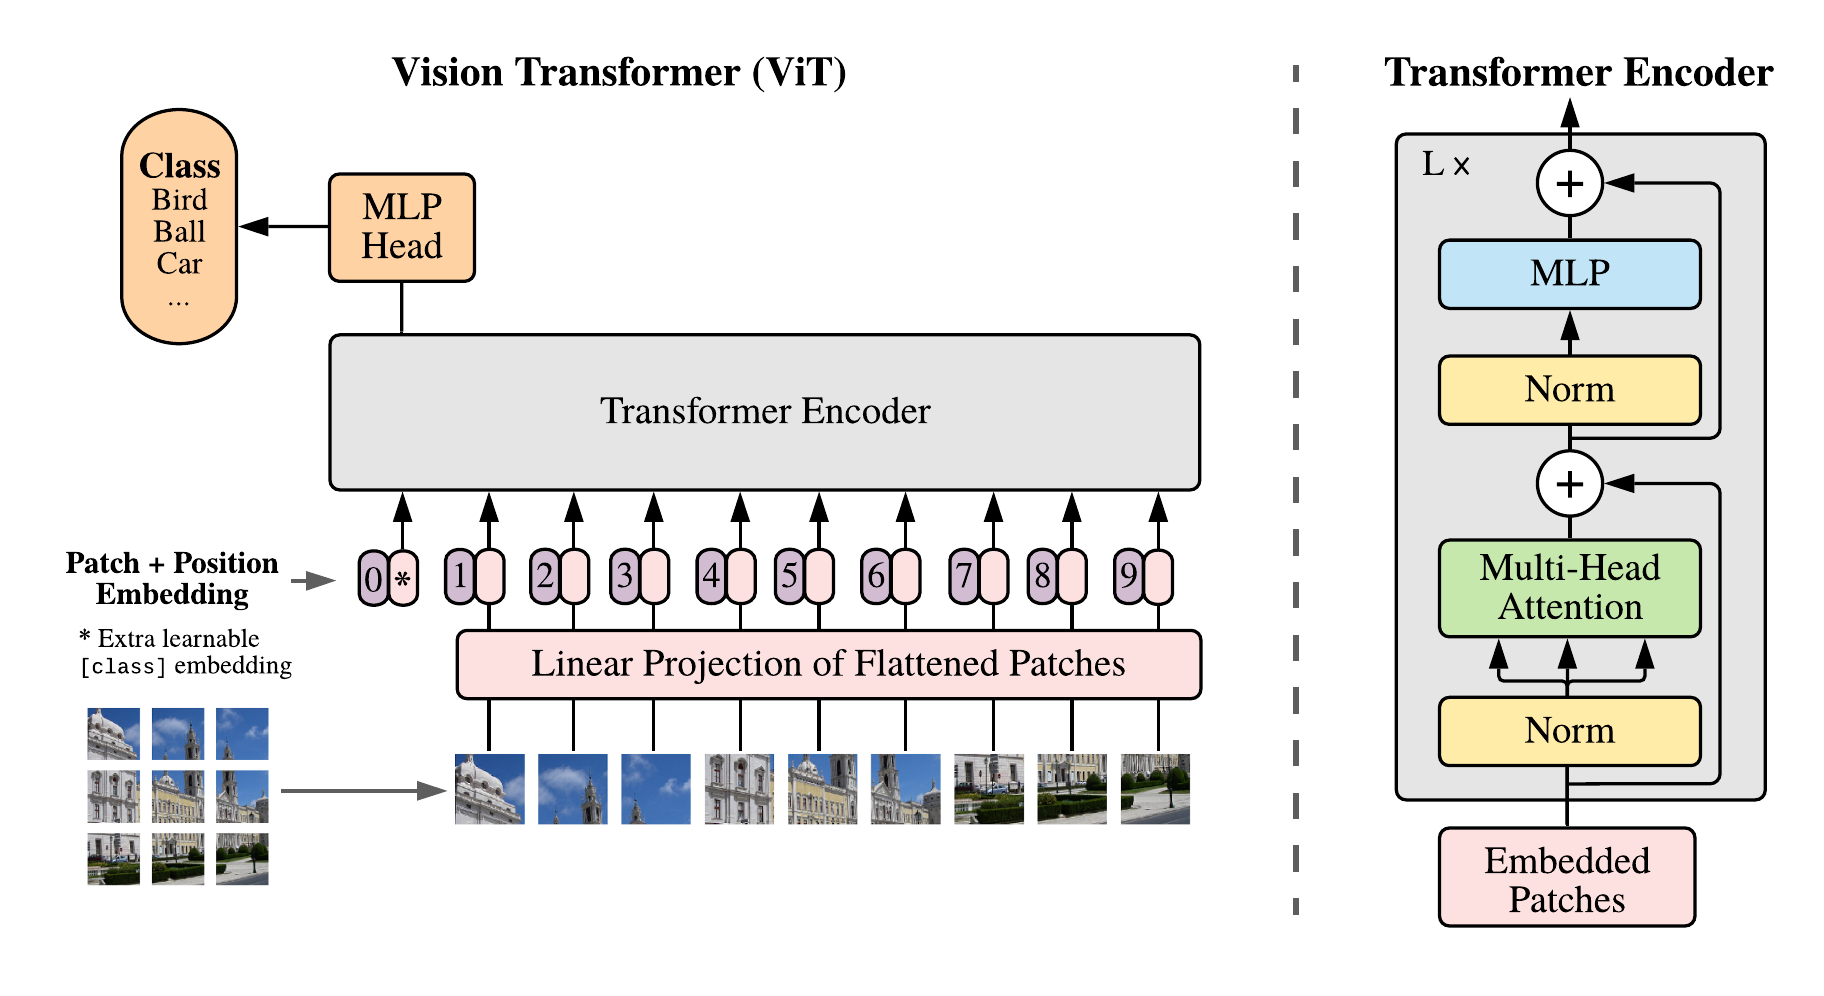
\includegraphics[width=1\textwidth]{vision-transformer-arch.png}
    \end{figure}

\end{frame}

\begin{frame}
    \frametitle{Експериментальні дослідження}
    \begin{itemize}
        \item Датасети ImageNet, CIFAR-10, Oxford-IIIT Pets,
        Oxford Flowers-102, VTAB (19 задач)
        \item 86, 307, 632 мільйонів параметрів відовідно для моделей
        \item Тисячі процесорних днів на TPUv3
    \end{itemize}

\end{frame}

\begin{frame}
    \frametitle{Експериментальні дослідження}
    \begin{figure}[H]
        \centering
        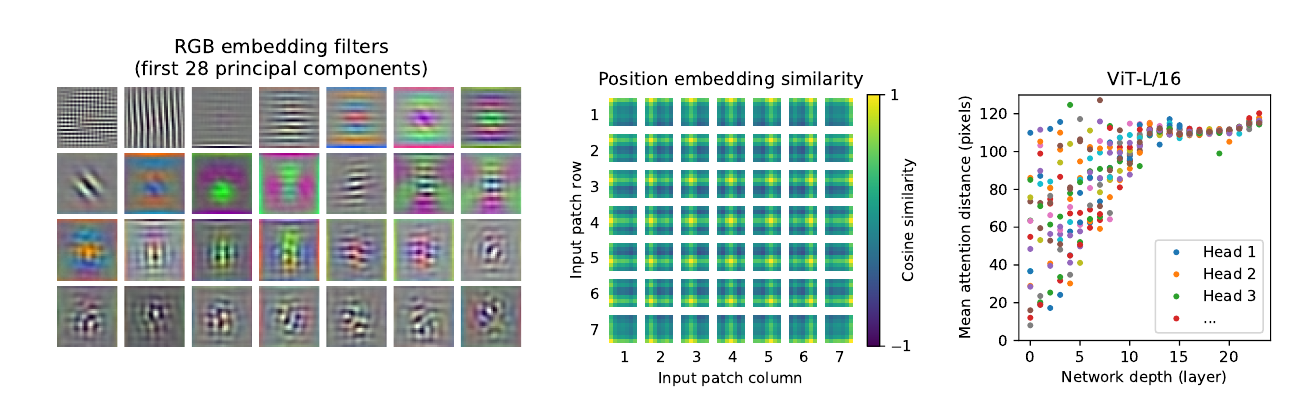
\includegraphics[width=1\textwidth]{filters.png}
    \end{figure}

\end{frame}

\begin{frame}
    \frametitle{Експериментальні дослідження}
    \begin{figure}[H]
        \centering
        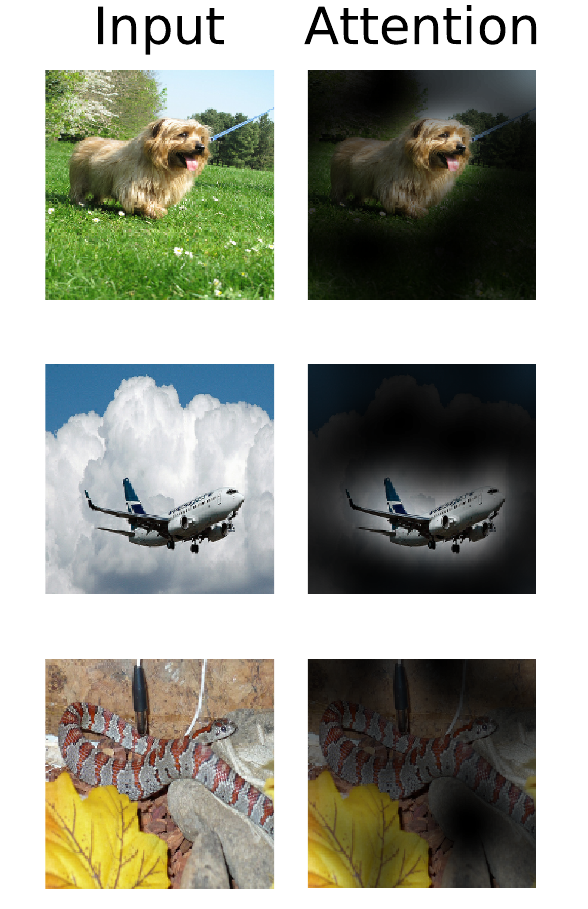
\includegraphics[width=0.4\textwidth]{attention-repr.png}
    \end{figure}

\end{frame}

\begin{frame}
    \frametitle{Висновки}
    Трансформери не використовують ні рекурентність, ні згортковість,
    та досягають (і в деяких випадках перевершує) спеціалізовані архітектури.

    Отже, трансформери можуть успішно використовуватися для вирішення
    задач обробки зображень, якщо є достатньо даних та
    обчислювальних ресурсів.

\end{frame}

\end{document}

% \begin{frame}
%     \frametitle{Організація бази даних}
%     \inputminted[breaklines,linenos=true]{yaml}{sample.yaml}
% \end{frame}

% \begin{frame}
%     \frametitle{Архітектура трансформерів}
%     \begin{figure}[H]
%         \centering
%         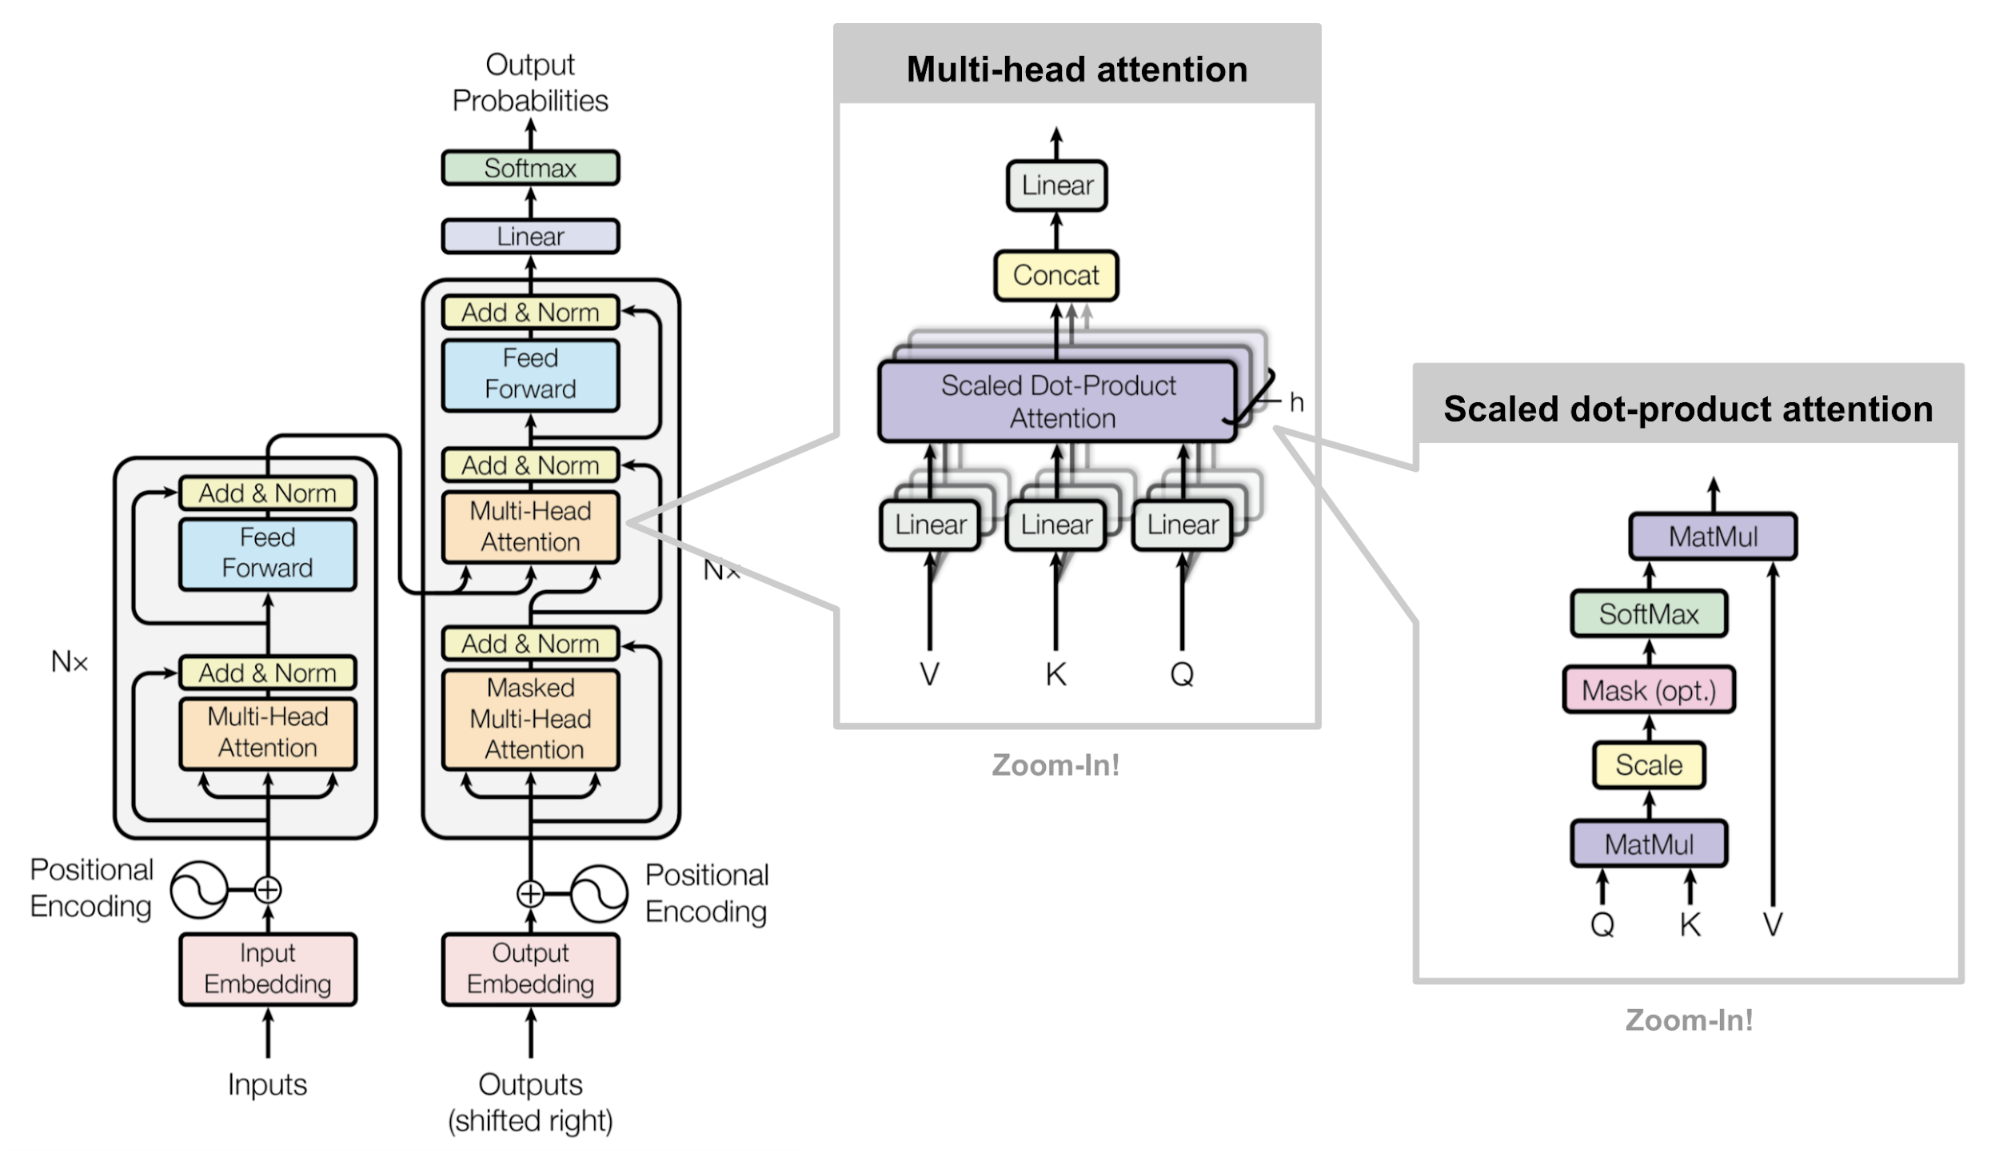
\includegraphics[width=0.5\textwidth]{transformer.png}
%     \end{figure}
% \end{frame}

% \begin{frame}
%     \frametitle{Шар уваги}
%     \begin{figure}[H]
%         \centering
%         \includegraphics[width=0.6\textwidth]{attention_layer.png}
%     \end{figure}
% \end{frame}